\chapter{Conceitos Básicos}

Esta seção tem por objetivo o estabelecimento dos conceitos básicos necessários ao entendimento do restante do trabalho. Não pretende-se aqui fazer uma explicação extensiva e profunda sobre os conceitos expostos, mas sim uma breve introdução, deixando os detalhes para serem procurados pelo leitor nas respectivas referências.

%%%%%%%%%%%
\section{Sistema Operacional}
Tanenbaum define sistemas operacionais sob duas perspectivas \cite{tanenbaum}:

\textbf{SO como uma máquina extendida:}
Programar ao nível de linguagem de máquina pode ser um tanto desastroso e desnecessariamente complicado. Por exemplo, na arquitetura PD765, o controlador de um disquete possui 16 comandos de controle, sendo os mais básicos os comandos WRITE e READ. Cada um destes comandos requerem 13 parâmetros, codificados em 9 bytes, parâmetros estes que específicam o endereço do bloco a ser lido, número de setores por trilha, modo de gravação desejada, etc.

Certamente um programador não quer ter que lidar com esse tipo de detalhe, e no lugar ele gostaria apenas de ter uma simples abstração de arquivos que podem ser abertos, editados, salvos e fechados.
O programa que procura esconder estes detalhes sórdidos é o sistema operacional, que procura abstrair o gerenciamento de arquivos, assim como detalhes sobre tratamento de interrupções, timers, gerenciamento de memória e qualquer outro detalhe de baixo nível, fazendo assim o programador ter a ilusão de estar interagindo com uma máquina mais simples e de mais alto nível.

\textbf{SO como um gerenciador de recursos:}
Diferentes processos competem entre si por utilizar os recursos do sistema. Estes processos precisam compartilhar entre si memória, tempo na CPU, dispositivos de entrada e saída, impressoras, etc. O programa responsável por conciliar as necessidades de cada processo, gerenciando os recursos da máquina de forma organizada e que atenda à todas as requisições por eles é, também, o sistema operacional.

\subsection{Processo}
Um processo basicamente é um programa \emph{em execução}, incluindo o seu \emph{program counter}, registradores e variáveis \cite{tanenbaum}. Cada processo possui um espaço de endereçamento próprio e individual, estando protegidos (e impedidos) de acessarem a porção de memória alocada para os demais processos. Cada processo executa na CPU por um certo intervalo de tempo, e então, caso não tenha terminado sua execução, esta é interrompida pelo escalonador de processos (veja seção \ref{escalonador}) para que a CPU possa ser usada por outro processo.

\subsection{Thread}
Todo processo está rodando pelo menos uma thread, e um conjunto de threads pode pertencer ao mesmo processo (toda thread pertence à algum processo). Cada thread pode executar independentemente, de forma pseudoparalela
\footnote{Em uma arquitetura de processador com apenas um núcleo, todos os processos e threads executam na realidade sequencialmente, entretanto parecem ser executadas paralelamente devido à pequena fatia de tempo que cada processo/thread possui para executar, por isto chamamos isto de pseudoparalelismo. Mesmo em arquiteturas de multiplos núcleos o paralelismo ``verdadeiro'' ainda não acontece com frequência, já que basta existirem mais processos/threads do que o número de núcleos para que estes tenham que ser sequenciados.}
, entretanto cada thread compartilha do espaço de endereçamento do processo ao qual pertencem. Cada thread possui seu próprio contexto, isto é, o estado de seus registradores (incluindo o \emph{program counter}, pilha e etc).
A vantagem de threads sobre processos é que a comunicação entre threads de um mesmo processo é muito mais rápida que a comunicação intraprocessos, e criar uma thread é mais rápido que criar um processo também.

\subsection{Escalonador}
\label{escalonador}

Um escalonador de processos (ou threads) é responsável por garantir que cada processo/thread consiga executar por algum determinado tempo na CPU. Existem diversos algoritmos de escalonamento, vários deles tendo sido implementados no EPOS. De acordo com Tanenbaum, há cinco dimensões que um escalonador deve levar em consideração em sua política de escalonamento \cite{tanenbaum}:

\begin{enumerate}
\item \textbf{Justiça (Fairness):} Assegurar que cada processo consiga executar por um tempo justo na CPU.
\item \textbf{Eficiência:} Tentar manter a CPU ocupada pela maior parte do tempo.
\item \textbf{Tempo de Resposta:} Minimizar o tempo de reposta para aplicações interativas.
\item \textbf{Turnaround:} Minimizar o tempo que processos \emph{batch} precisam esperar para executar.
\item \textbf{Vazão (throughput):} Maximizar a quantidade de tarefas realizadas por unidade de tempo.
\end{enumerate}

Claro que alguns destes itens são contraditórios entre si, por isto a escolha de um algoritmo de escalonamento depende da aplicação e carga de trabalho que o sistema pretende lidar.

% TODO Escalonadores de tempo real

%%%%%%%%%%%%%%%
\section{Sistema Embarcado}

É cada vez mais difícil definir o que é um sistema embarcado. Hoje sistemas embarcados estão em todos os lugares, eles acionam motores, freios, cintos de segurança, airbags, sistemas de audio em um carro. Eles codificam digitalmente voz e constroem sinais de radio e enviam eles de um celular para uma estação. Eles controlam microondas, ar-condicionados, semáforos, etc.

Existem sistemas embarcados dos mais diversos tamanhos e capacidades, desde aqueles com um \emph{clock} de poucos KHz, até processadores com GHz. Podemos dizer o que \emph{não} é um sistema embarcado: Notebooks, desktop, servidores e supercomputadores. É arriscar incorrer em erro tentar dar uma definição mais precisa \cite{leeseshia}.

%%%%%%%%%%%%%%%
\section{Sistemas de Tempo Real}

Sistemas de tempo real são definidos como aqueles sistemas nos quais a corretude geral do sistema depende tanto da corretude funcional (produzir o resultado correto) quanto a corretude temporal (produzir o resultado dentro do tempo máximo de tolerância). A corretude temporal é pelo menos tão importante quanto a corretude funcional \cite{realtime}. Ou seja, cada tarefa não somente deve produzir o resultado correto, mas também produzi-lo dentro de um intervalo de tempo predeterminado. Note que nem todos os sistemas de tempo real são sistemas embarcados, apesar de existir uma grande área em comum \footnote{Um sistema que oferece um serviço de \emph{streaming} de vídeo, por exemplo, é um sistema \emph{soft real-time}, mas não necessariamente embarcado.}\cite{realtime}. Os sistemas de tempo real podem ser classificados em duas categorias:

\begin{description}
	\item[Hard real-time] Nesta categoria, as tarefas dos sistemas devem necessariamente ser concluídas dentro do prazo, do contrário a resposta da tarefa já não faz mais sentido, e esta perda de prazo pode causar uma falha catastrófica do sistema, possivelmente causando grande prejuízo e até mesmo por vidas humanas em risco.
	\item[Soft real-time] Estes sistemas também precisam que suas tarefas sejam concluídas dentro do prazo, entretanto há certa tolerancia à atrasos, e no lugar de causar uma falha no sistema, a sucessiva perda de prazos costuma causar degradação do desempenho do sistema.
\end{description}

Exemplos de sistemas \emph{hard real-time} são vários. Imagine um sistema de detecção de mísseis, e que procura abater estes mísseis atirando neles. Fica claro que o tempo entre a detecção e a ação (atirar no míssil) está limitada à uma certa janela de tempo, e que a perda dessa janela de tempo pode resultar em ser acertado por um míssil \cite{realtime}.

Por outro lado, podemos imaginar também um reprodutor de vídeo. Cada \emph{frame} deve ser decodificado dentro de certa janela de tempo, do contrário aquele quadro pode não mais fazer sentido. Entretanto estes sistemas são tolerantes à perda de alguns quadros, portanto uma demora na codificação resulta numa degradação no desempenho (menor taxa de quadros por segundo), mas não evitam do vídeo não ser mais reproduzível. Este é um exemplo de sistema \emph{soft real-time}.

\section{Exceções e Interrupções}
Na terminologia adotada neste trabalho, uma exceção é um evento inesperado, que interrompe o processando normal do programa, fazendo o registrador PC apontar para uma região específica de memória, onde o tratador daquela exceção reside. Estas exceções incluem erros de permissão de leitura de certa parte da memória, tentativa de execução de uma instrução inválida (mal formada), etc.

Interrupções são bastante semelhantes à exceções. Elas param o fluxo normal de processamento, e também fazem com que a próxima instrução executada seja aquela numa região pré determinada da memória onde está o tratador daquela interrupção. A diferença esta no fato de interrupções poderem ser mascaradas, desativadas e gerenciadas pelo controlador de interrupção, enquanto não há controle sobre a execução das exceções (não são passíveis de desativação). Outra diferença, mais conceitual, é o fato que interrupções em geral são desejáveis e frequentemente necessárias para o funcionamento do sistema, enquanto exceções ocorrem apenas quando algo imprevisto é executado (como a execução de uma área de memória que não possui instruções executáveis).

A princípio, do ponto de vista do processador, uma interrução não tem muita diferença de uma exceção, por isto que no primeiro nível a interrupção é pré processada por um tratador de exceções, para então ser encaminhada para um tratador de interrupções (como mostra a figura \ref{fig:exception_handling}).


\section{ADESD}

ADESD (\emph{Application-Oriented System Design}) é um método de modelar de sistemas orientados à aplicação, em contrapartida aos sistemas operacionais de propósito geral.
Sistemas operacionais de propósito geral criam vários serviços e abstrações que acabam sendo nunca usados pela aplicação, e em alguns casos não oferecendo outras que a aplicação necessitaria \cite{guto_thesis}. Deste modo, no ADESD, o sistema se adapta à aplicação, e não a aplicação que deve se adaptar ao sistema. O EPOS é um sistema operacional criado usando esta perspectiva. Nas subseções seguintes será discutido algumas das técnicas usadas neste modelo, e que são exploradas durante o trabalho. Note que esta discussão é retomada no capítulo \ref{ch:epos}.

\subsection{Componente}
Um conceito bastante usado em ADESD é a noção de componente, um design baseado em componentes oferece meios para alcançar um SO orientado à aplicação \cite[p.~4]{guto_thesis}. Não há um consenso sobre como definir o que é um componente, Grady Booch define como ``Um componente reusável de software é um módulo logicamente coeso, fracamente aclopado que denota uma única abstração'', entretanto há muitas outras formas de definir isto.


\subsection{Metaprogramação estática}
Metaprograma é um program que representa e manipula outros programas ou eles próprios \cite{generative}.
Com metaprogramação é possível fazer-se loops (através de recursão), e condicionais (como o \verb+IF+ discutido abaixo), fazendo com que metaprogramas tenham equivalência à máquina de turing \cite{generative}. De fato, a linguagem de metaprogramação do C++ pode ser vista como uma linguagem funcional que tem sua execução em tempo de compilação. Pode-se fazer muitas estruturas metaprogramadas, inclusive listas, árvores e etc, entretanto nesta seção será mostrado apenas o funcionamento básico de um \verb+IF+ metaprogramado, pois este é bastante usado no código do EPOS. Para um maior entendimento sobre o assunto, fica aqui recomendado o livro referenciado \cite{generative}.

A arquitetura do EPOS usa com frequência metaprogramação estática para, em tempo de compilação, selecionar a arquitetura, bem como cada componente que será ou não utilizado. Por exemplo, podemos definir um \verb+if+ estático para selecionar de qual classe a classe Chronometer irá derivar. Primeiramente a definição do \verb+if+:

\begin{lstlisting}
template<bool condition, typename Then, typename Else>
struct IF
{
    typedef Then Result;
};
\end{lstlisting}

Este template, a princípio, nada mais faz do que tomar 3 parâmetros e então criar um tipo chamado \verb+Result+ igual ao segundo parâmetro, contudo, se fizermos uma especialização deste template, ele passa ser útil:

\begin{lstlisting}
template<typename Then, typename Else>
struct IF<false, Then, Else>
{
    typedef Else Result;
};
\end{lstlisting}


Com esta especialização, toda vez que o primeiro parâmetro resolver-se como falso, \verb+Result+ será definido como o terceiro parâmetro. Temos, portanto, um \verb+if+ metaprogramado funcional, agora voltemos ao exemplo do cronômetro.

Suponha que caso a arquitetura não seja multicore, e nos traits o TSC (\emph{time stamp clock}) esteja ativo, então deseja-se que Chronometer derive de TSC\_Chronometer, do contrário de Alarm\_Chronometer.

Isto pode ser feito usando nosso \verb+if+ metaprogramado da seguinte forma:

\begin{lstlisting}
class Chronometer: public
IF<Traits<TSC>::enabled && !Traits<System>::multicore,
TSC_Chronometer, Alarm_Chronometer>::Result
{/*class body*/};
\end{lstlisting}

Deste modo, \verb+Chronomometer+ derivará de \verb+IF::Result+, que será resolvido como TSC\_Chronometer ou Alarm\_Chronometer. Note que esse exemplo também mostra um uso do Traits, onde para descobrir se o TSC está ativo, bastou ler a constante \verb+Traits<TSC>::enabled+, e, para saber se o sistema é multicore, bastou ler \verb+Traits<System>::multicore+. Todo esse processamento causa zero \emph{overhead} em tempo de execução.

\subsection{Traits}

O uso de traits é uma técnica de metaprogramação estática para associar informações aos objetos em tempo de compilação. Por exemplo, uma matriz metaprogramada pode necessitar saber sua dimensão em tempo de compilação. No EPOS, por exemplo, no momento de criação da heap, e de inicialização da MMU, é necessário obter-se informações a respeito do mapeamento de memória do EPOS; estas informações são obtidas através do uso de traits.

Há basicamente 3 maneiras de definirmos traits \cite{generative}:

\begin{description}
\item[Traits como membro da classe:] Forma mais simples de definir-se um trait. Esta técnica basicamente consiste em criar-se constantes e tipos dentro da própria classe que os usa. Esta tecnica é muitas vezes usada sem o programador ter sequer conhecimento que está usando traits.

\item[Classes de traits:] Quando um tipo pode ter muitas características, e pode ser conveniente encapsulá-las numa única classe.

\item[Templates de Traits:] Consiste em definir uma classe de templates para gerenciar uma família de tipos. Esta é a técnica usada no EPOS, e será discutida melhor abaixo.

Nesta técnica, cria-se uma classe genérica, para que esta seja especializada por cada tipo que precisar de traits. Por exemplo, podemos fazer uma classe genérica \verb+number+, para associar informações sobre tipos numéricos, e então especializar esta classe para os diferentes tipos, como \verb+int+, \verb+long+, etc:

\begin{lstlisting}
template<class T>
class number {
public:
	static const bool specialized = false;
	static const unsigned long max = 0;
	static const unsigned long min = 0;
	static const bool sig = false; //Numero com sinal
};
template<>
class number<int> {
public:
	static const bool specialized = true;
	static const unsigned long max = 2147483647;
	static const long min = -2147483648;
	static const bool sig = true;
};
template<>
class number<unsigned long> {
public:
	static const bool specialized = true;
	static const unsigned long max = 4294967296;
	static const long min = 0;
	static const bool sig = false;
};
#include<iostream>
int main(){
	//exemplo de uso
	if(number<int>::specialized)
		std::cout << number<int>::min << std::endl;
	else
		std::cout << "Sem informacoes sobre int\n";
	
	return 0;
}
\end{lstlisting}

Neste exemplo, poderia-se especializar os demais tipos da linguagem C++, assim como adicionar novos atributos à estas especializações. Note que deste modo é possível centralizar num único arquivo várias características de vários tipos distintos, de forma organizada, de fácil manutenção e edição. No EPOS, os mais diversos componentes do SO podem ser configurados facilmente através dos traits; veja a seção \ref{sec:traits} para mais detalhes.
\end{description}

\subsection{Interface Infladas: } Um conceito da ADESD é a Interface Inflada. %http://www.inf.ufsc.br/~guto/publications/aoos.pdf
Em sistemas orientados à aplicação, famílias de abstrações são frequentemente tratadas como entidades únicas, algo que pode ser vantajoso para o programador da aplicação, já que este não precisaria se preocupar com qual membro em específico desta família ele precisaria usar \cite{guto_thesis}.

Interface inflada basicamente é uma interface que declara os métodos de todas as classes que derivam dela, exportanto assim todos os métodos daquela família de abstrações, como mostra a figura \ref{fig:inflated}. Deste modo, o desenvolvedor de aplicativo poderia escrever a aplicação inteira em termos da interface inflada, relegando a tarefa de configuração do sistema a um utilitário automatizado. Tal utilitário poderia, através de uma análise sintática do código fonte, escolher quais os membros mais apropriados da família exportada serão associados no momento da compilação \cite[p.~56]{guto_thesis}.

\begin{figure}[ht!]
	\label{fig:inflated}
    \centering
    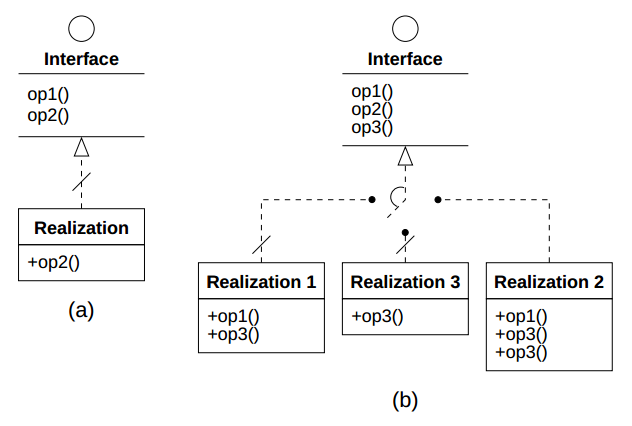
\includegraphics[width=7.5cm]{figuras/inflated_interface}
    \caption{Exemplos de uso de interfaces infladas \cite{guto_thesis}.}
\end{figure}




%%%%%%%%%%%%%%
\section{Arquitetura de microprocessadores}

Existe uma vasta variedade de sistemas embarcados, de modo que é difícil delinear características que são comuns a todos, portanto nas seções abaixo são colocados alguns conceitos que estão presentes na plataforma escolhida para este trabalho.

\subsection{Registradores Mapeados em Memória}
Uma maneira usada para se comunicar, configurar e ler o estado de um dado componente de hardware é através da leitura e/ou escrita em registradores mapeados em memória. Um registrador mapeado em memória basicamente é uma região fixa da memória, onde uma escrita naquela posição indica uma escrita no registrador lá mapeado.
Exemplificando, a UART da Zedboard possui um registrador chamado rcvr\_timeout\_reg0, responsável por indicar quantos ciclos\footnote{Na realidade é o número de baud\_samples que se passaram.} a UART deve esperar um novo caractere chegar antes de emitir uma interrupção de \emph{timeout}. Este registrador está mapeado na posição de memória 0xE000001C para a UART0. Portanto, para configurar que o número de ciclos esperado seja de 20, basta escrever este número naquela posição. Uma maneira de fazer esta escrita, por exemplo, em C/C++, é: \verb+*((unsigned long*)0xE000001C) = 20;+.

%%%%
%\section{Orientação a Objetos}
%Programação orientada a objetos é um método de implementação no qual programas são organizados como coleções cooperantes de objetos, cada qual representa uma instância de alguma classe, sendo que estas classes são todas membros de uma hierarquia de classes unidas por relações de herança \cite{OOAD}.

%%%%


\subsection{MMU} %http://epos.lisha.ufsc.br/EPOS+User+Guide#MMU
A MMU (\emph{Memory Managemed Unit}) é um componente responsável por gerenciar a memória de um sistema. É este componente o responsável por traduzir o endereçamento lógico (memória virtual) em endereçamento físico (memória física). Uma das principais vantagens de seu uso é a possibilidade de proteção de memória (entre processos e SO) e facilitação da escrita de aplicativos, pois estes não precisam levar em consideração o mapa de memória do SO.

\subsection{UART}
A UART (Universal Asynchronous Receiver/Transmitter) é um componente que trata da saída e entrada serial do sistema, portanto sendo o componente responsável por transmitir e receber caracteres, sendo necessário para impressão em tela, o que pode ser feito por via USB (usado principalmente para depuração do código). As duas principais funções na classe da UART dentro do EPOS são justamente a put e get, para impressão e leitura de caractere, respectivamente. O Zynq possui duas UARTs.


\subsection{\emph{Timer}}

\emph{Timer} é um componente de hardware que pode ser configurado para contar um certo número de ciclos. Ao fim da contagem o \emph{timer} emite uma interrupção, que então o processador pode tratar. Este componente é fundamental para um escalonador de processos e \emph{threads}.



\section{Ambiente de Desenvolvimento}

O ambiente de desenvolvimento usado para o porte foi o qemu para ARM (\verb+qemu-system-arm+) modificado pela Xilinx, para executar o EPOS num ambiente virtualizado (emulado), pois assim pode-se usar ferramentas como o GDB para a depuração do código de forma rápida. O uso do GDB foi fundamental para o desenvolvimento, já que com ele era possível imprimir o valor de cada registrador em um dado ponto da execução, verificar a memória, executar instruções específicas e etc. Para compilar o EPOS foi usado \emph{cross-compilers} para ARM. As flags usadas para criar um ambiente de depuração com o qemu e o GDB foram as seguintes (com cada comando feito em um terminal diferente):
%\hspace*{-1.0cm}\vbox{
\begin{verbatim}
./qemu-system-arm -kern-dtb ./xilinx_zynq.dtb \
    -no-reboot -nographic -smp 2 -machine xilinx-zynq-a9 \
    -cpu cortex-a9 -kernel img/panda_app -m 512 \
    -fda img/panda_app.img

arm-none-eabi-gdb -ex "target remote :1234"
\end{verbatim}
%}

O hardware real também estava disponível, e foi usado quando o qemu não produzia resultados confiáveis. Com o hardware real, para a depuração do código foi usado o JTAG.
Para carregar a imagem do SO na placa, foi usada a ferramenta da Xilinx \verb-xmd-, sendo que esta ferramenta trata de fazer o processador apontar para o ponto de entrada da imagem carregada, de tal modo que é possível conectar o GDB através da porta aberta pelo \verb+xmd+, e então executar através do GDB.
